%!TEX TS-program = xelatex
\documentclass[10pt,oneside]{article}
\usepackage[fontsize=9pt]{scrextend}

\usepackage[english]{babel}

\usepackage{amsmath,amssymb,amsfonts}
\usepackage[utf8]{inputenc}
\usepackage[T1]{fontenc}
\usepackage{stix2}
\usepackage[scaled]{helvet}
\usepackage[scaled]{inconsolata}

\usepackage{lastpage}

\usepackage{setspace}

\usepackage{ccicons}

\usepackage[hang,flushmargin]{footmisc}

\usepackage{geometry}

\setlength{\parindent}{0pt}
\setlength{\parskip}{6pt plus 2pt minus 1pt}

\usepackage{fancyhdr}
\renewcommand{\headrulewidth}{0pt}\providecommand{\tightlist}{%
  \setlength{\itemsep}{0pt}\setlength{\parskip}{0pt}}

\makeatletter
\newcounter{tableno}
\newenvironment{tablenos:no-prefix-table-caption}{
  \caption@ifcompatibility{}{
    \let\oldthetable\thetable
    \let\oldtheHtable\theHtable
    \renewcommand{\thetable}{tableno:\thetableno}
    \renewcommand{\theHtable}{tableno:\thetableno}
    \stepcounter{tableno}
    \captionsetup{labelformat=empty}
  }
}{
  \caption@ifcompatibility{}{
    \captionsetup{labelformat=default}
    \let\thetable\oldthetable
    \let\theHtable\oldtheHtable
    \addtocounter{table}{-1}
  }
}
\makeatother

\usepackage{array}
\newcommand{\PreserveBackslash}[1]{\let\temp=\\#1\let\\=\temp}
\let\PBS=\PreserveBackslash

\usepackage[breaklinks=true]{hyperref}
\hypersetup{colorlinks,%
citecolor=blue,%
filecolor=blue,%
linkcolor=blue,%
urlcolor=blue}
\usepackage{url}

\usepackage{caption}
\setcounter{secnumdepth}{0}
\usepackage{cleveref}

\usepackage{graphicx}
\makeatletter
\def\maxwidth{\ifdim\Gin@nat@width>\linewidth\linewidth
\else\Gin@nat@width\fi}
\makeatother
\let\Oldincludegraphics\includegraphics
\renewcommand{\includegraphics}[1]{\Oldincludegraphics[width=\maxwidth]{#1}}

\usepackage{longtable}
\usepackage{booktabs}

\usepackage{color}
\usepackage{fancyvrb}
\newcommand{\VerbBar}{|}
\newcommand{\VERB}{\Verb[commandchars=\\\{\}]}
\DefineVerbatimEnvironment{Highlighting}{Verbatim}{commandchars=\\\{\}}
% Add ',fontsize=\small' for more characters per line
\usepackage{framed}
\definecolor{shadecolor}{RGB}{248,248,248}
\newenvironment{Shaded}{\begin{snugshade}}{\end{snugshade}}
\newcommand{\KeywordTok}[1]{\textcolor[rgb]{0.13,0.29,0.53}{\textbf{#1}}}
\newcommand{\DataTypeTok}[1]{\textcolor[rgb]{0.13,0.29,0.53}{#1}}
\newcommand{\DecValTok}[1]{\textcolor[rgb]{0.00,0.00,0.81}{#1}}
\newcommand{\BaseNTok}[1]{\textcolor[rgb]{0.00,0.00,0.81}{#1}}
\newcommand{\FloatTok}[1]{\textcolor[rgb]{0.00,0.00,0.81}{#1}}
\newcommand{\ConstantTok}[1]{\textcolor[rgb]{0.00,0.00,0.00}{#1}}
\newcommand{\CharTok}[1]{\textcolor[rgb]{0.31,0.60,0.02}{#1}}
\newcommand{\SpecialCharTok}[1]{\textcolor[rgb]{0.00,0.00,0.00}{#1}}
\newcommand{\StringTok}[1]{\textcolor[rgb]{0.31,0.60,0.02}{#1}}
\newcommand{\VerbatimStringTok}[1]{\textcolor[rgb]{0.31,0.60,0.02}{#1}}
\newcommand{\SpecialStringTok}[1]{\textcolor[rgb]{0.31,0.60,0.02}{#1}}
\newcommand{\ImportTok}[1]{#1}
\newcommand{\CommentTok}[1]{\textcolor[rgb]{0.56,0.35,0.01}{\textit{#1}}}
\newcommand{\DocumentationTok}[1]{\textcolor[rgb]{0.56,0.35,0.01}{\textbf{\textit{#1}}}}
\newcommand{\AnnotationTok}[1]{\textcolor[rgb]{0.56,0.35,0.01}{\textbf{\textit{#1}}}}
\newcommand{\CommentVarTok}[1]{\textcolor[rgb]{0.56,0.35,0.01}{\textbf{\textit{#1}}}}
\newcommand{\OtherTok}[1]{\textcolor[rgb]{0.56,0.35,0.01}{#1}}
\newcommand{\FunctionTok}[1]{\textcolor[rgb]{0.00,0.00,0.00}{#1}}
\newcommand{\VariableTok}[1]{\textcolor[rgb]{0.00,0.00,0.00}{#1}}
\newcommand{\ControlFlowTok}[1]{\textcolor[rgb]{0.13,0.29,0.53}{\textbf{#1}}}
\newcommand{\OperatorTok}[1]{\textcolor[rgb]{0.81,0.36,0.00}{\textbf{#1}}}
\newcommand{\BuiltInTok}[1]{#1}
\newcommand{\ExtensionTok}[1]{#1}
\newcommand{\PreprocessorTok}[1]{\textcolor[rgb]{0.56,0.35,0.01}{\textit{#1}}}
\newcommand{\AttributeTok}[1]{\textcolor[rgb]{0.77,0.63,0.00}{#1}}
\newcommand{\RegionMarkerTok}[1]{#1}
\newcommand{\InformationTok}[1]{\textcolor[rgb]{0.56,0.35,0.01}{\textbf{\textit{#1}}}}
\newcommand{\WarningTok}[1]{\textcolor[rgb]{0.56,0.35,0.01}{\textbf{\textit{#1}}}}
\newcommand{\AlertTok}[1]{\textcolor[rgb]{0.94,0.16,0.16}{#1}}
\newcommand{\ErrorTok}[1]{\textcolor[rgb]{0.64,0.00,0.00}{\textbf{#1}}}
\newcommand{\NormalTok}[1]{#1}

\newlength{\cslhangindent}
\setlength{\cslhangindent}{1.5em}
\newlength{\csllabelwidth}
\setlength{\csllabelwidth}{3em}
\newenvironment{CSLReferences}[3] % #1 hanging-ident, #2 entry spacing
 {% don't indent paragraphs
  \setlength{\parindent}{0pt}
  % turn on hanging indent if param 1 is 1
  \ifodd #1 \everypar{\setlength{\hangindent}{\cslhangindent}}\ignorespaces\fi
  % set entry spacing
  \ifnum #2 > 0
  \setlength{\parskip}{#2\baselineskip}
  \fi
 }%
 {}
\usepackage{calc} % for \widthof, \maxof
\newcommand{\CSLBlock}[1]{#1\hfill\break}
\newcommand{\CSLLeftMargin}[1]{\parbox[t]{\maxof{\widthof{#1}}{\csllabelwidth}}{#1}}
\newcommand{\CSLRightInline}[1]{\parbox[t]{\linewidth}{#1}}
\newcommand{\CSLIndent}[1]{\hspace{\cslhangindent}#1}\usepackage[table,dvipsnames]{xcolor}

\geometry{includemp,
            letterpaper,
            top=2.4cm,
            bottom=2.4cm,
            left=1.0cm,
            right=1.0cm,
            marginparwidth=5cm,
            marginparsep=1.0cm}

\usepackage[singlelinecheck=off]{caption}

\captionsetup{
  font={small},
  labelfont={bf},
  format=plain,
  labelsep=quad
}

\usepackage{floatrow}

\floatsetup[figure]{margins=hangright,
              facing=no,
              capposition=beside,
              capbesideposition={center,outside},
              floatwidth=\textwidth}

% \floatsetup[table]{margins=hangright,
%              facing=no,
%              capposition=beside,
%              capbesideposition={center,outside},
%              floatwidth=\textwidth}

\pagestyle{plain}

\setcounter{secnumdepth}{5}

\usepackage{titlesec}

\titleformat{\section}[block]
{\normalfont\large\sffamily}
{\thesection}{.5em}{\titlerule\\[.8ex]\bfseries}

\titleformat{\subsection}[runin]
{\normalfont\fontseries{b}\selectfont\filright\sffamily}
{\thesubsection.}{.5em}{}

\titleformat{\subsubsection}[runin]
{\normalfont\itshape\rmfamily\bfseries}{\thesubsubsection}{1em}{}

\fancypagestyle{firstpage}
{
   \fancyhf{}
   \renewcommand{\headrulewidth}{0pt}
   \fancyfoot[R]{\footnotesize\ccby}
   \fancyfoot[L]{\footnotesize\sffamily\today}
}

\fancypagestyle{normal}
{
  \fancyhf{}
  \fancyfoot[R]{\footnotesize\sffamily\thepage\ of \pageref*{LastPage}}
}

\usepackage{tikz}
\begin{document}
\tikz [remember picture, overlay] %
\node [shift={(-0.6in,1.1cm)},scale=0.2,opacity=0.4] at (current page.south east)[anchor=south east]{
\includegraphics{logo}};%
\pagestyle{normal}
\thispagestyle{firstpage}

\newcommand{\colorRule}[3][black]{\textcolor[HTML]{#1}{\rule{#2}{#3}}}

\noindent {\LARGE \textbf{\textsf{Dissimilarity of species interaction
networks: quantifying the effect of turnover and rewiring}}}

\medskip
\begin{flushleft}
{\small
%
\href{https://orcid.org/0000-0002-0735-5184}{Timothée\,Poisot}%
%
\,\textsuperscript{1,2,‡}
\vskip 1em
\textsuperscript{1}\,Université de Montréal; \textsuperscript{2}\,Québec
Centre for Biodiversity Sciences\\
\textsuperscript{‡}\,These authors contributed equally to the work\\
\vskip 1em
\textbf{Correspondance to:}\\
Timothée Poisot --- \texttt{timothee.poisot@umontreal.ca}\\
}
\end{flushleft}

\vskip 2em
\makebox[0pt][l]{\colorRule[CCCCCC]{2.0\textwidth}{0.5pt}}
\vskip 2em
\noindent

\marginpar{\vskip 1em\flushright
{\small{\bfseries Keywords}:\par
ecological network dissimilarity\\turnover partitioning\\species
interaction networks\\}
}


Despite having established its usefulness in the last ten years, the
decomposition of ecological networks in components allowing to measure
their \(\beta\)-diversity retains some methodological ambiguities.
Notably, how to quantify the relative effect of mechanisms tied to
interaction rewiring \emph{vs.} species turnover has been interpreted
differently by different authors. In this contribution, I present
mathematical arguments and numerical experiments that should (i)
establish that the decomposition of networks as it is currently done is
indeed fit for purpose, and (ii) provide guidelines to interpret the
values of the components tied to turnover and rewiring.




\vskip 2em
\makebox[0pt][l]{\colorRule[CCCCCC]{2.0\textwidth}{0.5pt}}
\vskip 2em

Ecological networks are variable both in time and space (Poisot \emph{et
al.} 2015; Trøjelsgaard \& Olesen 2016) - this variability motivated the
emergence of methodology to compare ecological networks, including in a
way that meshes with the core concept for the comparison of ecological
communities, namely \(\beta\)-diversity (Poisot \emph{et al.} 2012). The
need to understand network variability through partitioning in
components equivalent to \(\alpha\), \(\beta\), and \(\gamma\)
diversities is motivated by the prospect to further integrate the
analysis of species interactions to the analysis of species
compositions. Because species that make up the networks do not react to
their environment in the same way, and because interactions are only
expressed in subsets of the environments in which species co-occurr, the
\(\beta\)-diversity of networks may behave in complex ways, and its
quantification is likely to be ecologically informative.

Poisot \emph{et al.} (2012) and Canard \emph{et al.} (2014) have
suggested an approach to \(\beta\)-diversity for ecological networks
which is based on the comparison of the number of shared and unique
links among species within a pair of networks. Their approach
differentiates this sharing of links between those established between
species occurring in both networks, and those established with at least
one unique species. This framework is expressed as the decomposition
\(\beta_{wn} = \beta_{os} + \beta_{st}\), namely the fact that network
dissimilarity (\(\beta_{wn}\)) has a component that can be calculated
directly from the dissimilarity of interactions between shared species
(\(\beta_{os}\)), and a component that cannot (\(\beta_{st}\)).
Presumably, the value of these components for a pair of networks can
generate insights about the mechanisms involved in dissimilarity.

This approach has been widely adopted since its publication, with recent
examples using it to understand the effect of fire on pollination
systems (Baronio \emph{et al.} 2021); the impact of rewiring on
spatio-temporal network dynamics (Campos-Moreno \emph{et al.} 2021); the
effects of farming on rural and urban landscapes on species interactions
(Olsson \emph{et al.} 2021); the impact of environment gradients on
multi-trophic metacommunities (\textbf{Ohlmann2018MapImp?}); and as a
tool to estimate the sampling completeness of networks (Souza \emph{et
al.} 2021). It has, similarly, received a number of extensions,
including the ability to account for interaction strength (Magrach
\emph{et al.} 2017), the ability to handle probabilistic ecological
networks (Poisot \emph{et al.} 2016), and the integration into the Local
Contribution to Beta Diversity (Legendre \& De Cáceres 2013) approach to
understand how environment changes drive network dissimilarity (Poisot
\emph{et al.} 2017).

\begin{figure}
\hypertarget{fig:conceptual}{%
\centering
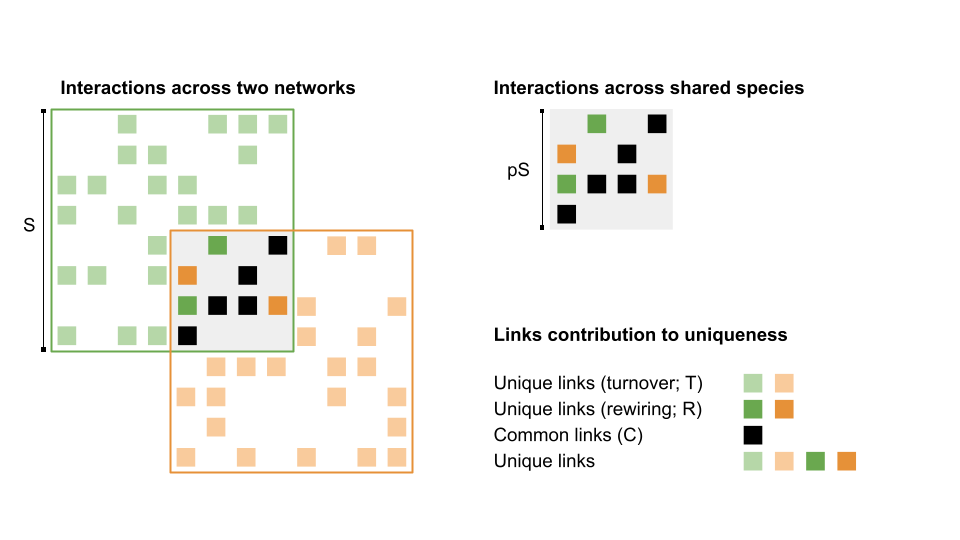
\includegraphics{figures/betadiv_response_figure.png}
\caption{TK}\label{fig:conceptual}
}
\end{figure}

Yet, the precise meaning of \(\beta_{st}\), namely the importance of
species turnover in the overall dissimilarity, has been difficult to
capture, and a source of confusion for some practitioners. This is not
particularly surprising, as this component of the decomposition responds
to unique species introducing their unique interactions both between
themselves, and with species that are common to both networks
fig.~\ref{fig:conceptual}. For this reason, it is important to come up
with guidelines for the interpretation of this measure, and how to use
it to extract ecological insights.

Furthermore, much like the definition of \(\beta\)-diversity in all its
forms is a contentious topic amongst community ecologists (see
\emph{e.g.} Tuomisto 2010), the \(\beta\)-diversity of networks has been
submitted to methodological scrutiny over the years. A synthesis of some
criticisms, related to the correct denominator to use to express the
proportion of different links, has recently been published (Fründ 2021).
It argues that the calculation of network dissimilarity terms as
originally outlined by Poisot \emph{et al.} (2012) is incorrect, as it
can lead to over-estimating the role of interactions between shared
species in a network (``rewiring''), and therefore underestimate the
importance of species turnover across networks. As mist-understanding
either of these quantities can lead to biased inferences about the
mechanisms generating network dissimilarity, it is important to assess
how the values (notably of \(\beta_{os}\), and therefore of
\(\beta_{st}\)) react to methodological choices.

Here, I present a mathematical analysis of the Poisot \emph{et al.}
(2012) method, explain how information about species turnover and link
rewiring can be extracted from its decomposition, and conduct numerical
experiments to guide the interpretation of the \(\beta\)-diversity
values thus obtained (with a specific focus on \(\beta_{st}\)). These
numerical experiments establish three core facts. First, the
decomposition adequately captures the relative roles of species turnover
and interaction rewiring; second, the decomposition responds to
differences in network structure (like connectance) as expected;
finally, the decomposition more accurately captures rewiring than the
proposed alternative using a different denominator put forth by Fründ
(2021).

\hypertarget{partitioning-network-dissimilarity}{%
\subsection{Partitioning network
dissimilarity}\label{partitioning-network-dissimilarity}}

The approach to quantifying the difference between pairs of networks
established in Poisot \emph{et al.} (2012) is a simple extension of the
overall method by Koleff \emph{et al.} (2003) for species dissimilarity
based on presence-absence data. The objects to compare, \(X_1\) and
\(X_2\), are partitioned into three values, \(a = |X_1 \cup X_2|\),
\(b = |X_2 \setminus X_1|\), and \(c = |X_1 \setminus X_2|\), where
\(|\dot|\) is the cardinality of set \(\dot\) (the number of elements it
contains), and \(\setminus\) is the set substraction operation. In the
perspective of species composition comparison, \(X_1\) and \(X_2\) are
the sets of species in either community, so that if
\(X_1 = \{x, y, z\}\) and \(X_2 = \{v, w, x, y\}\), we have
\(X_1 \cup X_2 = \{v, w, x, y, z\}\), \(X_1 \cap X_2 = \{x, y\}\),
\(X_2 \setminus X_1 = \{v, w\}\), and \(X_1 \setminus X_2 = \{z\}\). The
core message of Koleff \emph{et al.} (2003) is that the overwheling
majority of measures of \(\beta\)-diversity can be re-expressed as
functions that operate on the cardinality of these sets -- this allows
to focus on the number of unique and common elements, as outlined in
fig.~\ref{fig:conceptual}.

\hypertarget{re-expressing-networks-as-sets}{%
\subsubsection{Re-expressing networks as
sets}\label{re-expressing-networks-as-sets}}

Applying this framework to networks requires a few additional
definitions. Although ecologists tend to think of networks as their
adjacency matrix, this representation is far from optimal to get a solid
understanding of which elements should be counted as part of which set
when measuring network dissimilarity. For this reason, we need fall back
on the definition of a graph as a pair of sets, wherein
\(\mathcal{G} = (V, E)\). These two components \(V\) and \(E\) represent
vertices (nodes, species) and edges (interactions), where \(V\) is
specifically a set containing the vertices \(\mathcal{G}\), and \(E\) is
a set of ordered pairs, in which every pair is composed of two elements
of \(V\); an element \(\{i,j\}\) in \(E\) indicates that there is an
interaction \emph{from} species \(i\) to species \(j\) in the network
\(\mathcal{G}\).

In the context of networks comparison (assuming the networks to compare
are \(\mathcal{M}\) and \(\mathcal{N}\)), we can further decompose the
contents of these sets as

\[\mathcal{M} = (V_c \cup V_m, E_c \cup E_{sm} \cup E_{um}) \,,\]

and

\[\mathcal{M} = (V_c \cup V_n, E_c \cup E_{sn} \cup E_{un}) \,,\]

where \(V_c\) is the set of shared species, \(V_k\) are the species
belonging only to network \(k\), \(E_c\) are the shared edges, and
\(E_{sk}\) and \(E_{uk}\) are the interactions unique to \(k\)
involving, respectively, only species in \(V_c\), and at least one
species from \(V_k\).

\hypertarget{defining-the-partitions-from-networks-as-sets}{%
\subsubsection{Defining the partitions from networks as
sets}\label{defining-the-partitions-from-networks-as-sets}}

The metaweb (Dunne 2006), which is to say the entire regional species
pool and their interaction, can be defined as
\(\mathcal{M} \cup \mathcal{N}\) (this operation is commutative), which
is to say

\[\mathcal{M} \cup \mathcal{N} = (V_c \cup V_m \cup V_n, E_c \cup E_{sm} \cup E_{um} \cup E_{sn} \cup E_{un}) \,.\]

This operation gives us an equivalent to \(\gamma\)-diversity for
networks, in that the set of vertices contains \emph{all} species from
the two networks, and the set of edges contains \emph{all} the
interactions between these species. If, further, we make the usual
assumption that only species with at least one interaction are present
in the set of vertices, then all elements of the set of vertices are
present at least once in the set of edges, and the set of vertices can
be entire reconstructed from the set of edges. Although measures of
network \(\beta\)-diversity operate on interactions (not species), this
property is maintained at every decomposition we will describe next.

We can similarly define the intersection (similarly commutative) of two
networks:

\[\mathcal{M} \cap \mathcal{N} = (V_c, E_c)\,.\]

The decomposition of \(\beta\)-diversity from Poisot \emph{et al.}
(2012) uses these components to measure \(\beta_{os}\) (the interaction
dissimilarity between shared species, which Fründ (2021) terms
``rewiring''), and \(\beta_{wn}\) (the overall dissimilarity including
non-shared species). We can express the components \(a\), \(b\), and
\(c\) of Koleff \emph{et al.} (2003) as the cardinality of the following
sets:

\begin{longtable}[]{@{}llll@{}}
\toprule
Component & \(a\) & \(b\) & \(c\)\tabularnewline
\midrule
\endhead
\(\beta_{os}\) & \(E_c\) & \(E_{sn}\) & \(E_{sm}\)\tabularnewline
\(\beta_{wn}\) & \(E_c\) & \(E_{sn} \cup E_{un}\) &
\(E_{sm} \cup E_{um}\)\tabularnewline
\bottomrule
\end{longtable}

These decompositions are used to perform the calculations of
\(\beta\)-diversity in the \texttt{EcologicalNetworks.jl} package
(Banville \emph{et al.} 2021) for Julia, which I use for the following
numerical experiments.

\hypertarget{quantifying-the-importance-of-species-turnover}{%
\subsection{Quantifying the importance of species
turnover}\label{quantifying-the-importance-of-species-turnover}}

The difference between \(\beta_{os}\) and \(\beta_{wn}\) stems from the
species dissimilarity between \(\mathcal{M}\) and \(\mathcal{N}\), and
it is easier to understand the effect of turnover by picking a
dissimilarity measure to work as an exemplar. At this point, Fründ
(2021) introduce a confusin terminology in their work, stating that
S\o rensen's and Whittaker's measures of dissimilarity are the same in
the Koleff \emph{et al.} (2003) framework (they are not; in practice,
\(\beta_{Sor}=1-\beta_{w}\)), and (ii) noting Whittaker's measure as
\((b+c)/(2a+b+c)\), which in the Koleff \emph{et al.} (2003) framework
is, in fact, \(\beta_t\) (Wilson \& Shmida 1984). This does not change
the overall conclusions as these measures can be re-expressed to
converge to the same value. For the sake of consistency, I will use
\(\beta_t\) moving forward; it returns values in \([0,1]\), with \(0\)
meaning complete similarity, and \(1\) meaning complete dissimilarity.

\hypertarget{establishing-that-beta_wn-ge-beta_os}{%
\subsubsection{\texorpdfstring{Establishing that
\(\beta_{wn} \ge \beta_{os}\)}{Establishing that \textbackslash beta\_\{wn\} \textbackslash ge \textbackslash beta\_\{os\}}}\label{establishing-that-beta_wn-ge-beta_os}}

Based on a partition between three sets of cardinality \(a\), \(b\), and
\(c\),

\[\beta_t = \frac{b+c}{2a+b+c}\,.\]

So as to simplify the notation of the following section, I will
introduce a series of new variables. Let \(A = |E_c|\) be the number of
links that are identical between networks; \(S = |E_{sn} \cup E_{sm}|\)
be the number of links that are not shared, but only involve shared
species (\emph{i.e.} links from \(\mathcal{M}\cup\mathcal{N}\)
established between species from \(\mathcal{M}\cap\mathcal{N}\)); and
\(U = |E_{un} \cup E_{um}|\) the number of links that are not shared,
and involve at least one unique species. Adopting the perspective
developed in the previous section, wherein networks are sets and the
measures of \(\beta\)-diversity operates on these sets, highlights the
conceptual issue in the Fründ (2021) alternative normalization: they are
using components of the networks that are \emph{not} part of the
networks being compared.

There are two important points to note here. First, the number or
proportion of species that are shared is not involved in the
calculation. Second, the connectance of either network is not involved
in the calculation. That all links counted in \emph{e.g.} \(U\) come
from \(\mathcal{M}\), or that they are evenly distributed between
\(\mathcal{M}\) and \(\mathcal{N}\), has no impact on the result. This
is a desirable property of the approach: whatever quantitative value of
the components of dissimilarity can be interpreted in the light of the
connectance and species turnover \emph{without} any risk of circularity.
Therefore the argument of Fründ (2021), whereby the \(\beta_{os}\)
component should decrease with turnover, and be invariant to
connectance, does not hold: the very point of the approach is to provide
measures that can be interpreted in the light of connectance and species
turnover.

The final component of network dissimilarity in Poisot \emph{et al.}
(2012) is \(\beta_{st}\), \emph{i.e.} the part of \(\beta_{wn}\) that is
not explained by changes in interactions between shared species
(\(\beta_{os}\)), and therefore stems from species turnover. This
fraction is defined as \(\beta_{st} = \beta_{wn}-\beta_{os}\).

The expression of \(\beta_{st}\) does not involve a partition into sets
that can be plugged into the framework of Koleff \emph{et al.} (2003),
because the part of \(\mathcal{M}\) and \(\mathcal{N}\) that are
composed of their unique species cannot, by definition, share
interactions. One could, theoretically, express these as
\(\mathcal{M} \setminus \mathcal{N} = (V_m, E_{um})\) and
\(\mathcal{N} \setminus \mathcal{M} = (V_v, E_{un})\) (note the
non-commutativity here), but the dissimilarity between these networks is
trivially maximal for the measures considered.

Using the \(\beta_t\) measure of dissimilarity, we can re-write (using
the notation with \(A\), \(S\), and \(U\))

\[\beta_{os} = \frac{S}{2A+S}\,,\]

and

\[\beta_{wn} = \frac{S+U}{2A+S+U}\,.\]

Note that \(\beta_{os}\) has the form \(x/y\) with \(x = S\) and
\(y = 2A+S\), and \(\beta_{wn}\) has the form \((x+k)/(y+k)\), with
\(k = U\). As long as \(k \ge 0\), it is guaranteed that
\(\beta_{wn} \ge \beta_{os}\), and therefore that
\(0 \ge \beta_{st} \ge 1\); as \(A\), \(S\), and \(U\) are cardinalities
of sets, they are necessarily satisfying this condition.

We can get an expression for \(\beta_{st}\), by bringing \(\beta_{os}\)
and \(\beta_{wn}\) to a common denominator and simplifying the
numerator:

\[\beta_{st} = \frac{2AU}{(2A+S)(2A+S+U)}\,.\]

Note that this value varies in a non-monotonic way with regards to the
number of interactions that are part of the common set of species --
this is obvious when developing the denominator into

\[4A^2 + S^2 + 4AS + 2AU + SU\,,\]

As such, we expect that the value of \(\beta_{st}\) will vary in a
hump-shaped way with the proportion of shared interactions. For this
reason, Poisot \emph{et al.} (2012) suggest that
\(\beta_{st}/\beta{wn}\) (alt. \(1-\beta_{os}/\beta_{wn}\)) is a better
indicator of the \emph{relative} importance of turnover processes on
network dissimilarity. This can be calculated as

\[\frac{\beta_{st}}{\beta_{wn}} = \frac{2AU}{(2A+S)(2A+S+U)}\times\frac{S+U}{2A+S+U}\,,\]

which reduces to

\[\frac{\beta_{st}}{\beta_{wn}} = \frac{2AU}{(2A+S)(S+U)}\,.\]

The roots of this expression are \(A=0\) (the turnover of species has no
contribution to the difference between \(\beta_{wn}\) and \(\beta_{os}\)
if there are no shared species, and therefore no rewiring), and for
\(U = 0\) (the turnover of species has no contribution if all species
are shared).

\hypertarget{numerical-experiment-response-of-the-components-to-different-sources-of-network-variation}{%
\subsubsection{Numerical experiment: response of the components to
different sources of network
variation}\label{numerical-experiment-response-of-the-components-to-different-sources-of-network-variation}}

To illustrate the behavior of \(\beta_{st}\), I conducted a simple
numerical experiment in which two networks have the same number of
interactions \(L\) (recall from the previous section that we do not need
to set a number of species yet), and these interactions are partitionned
according to proportions \(p_s\) and \(p_r\) into shared (\(A\)),
rewired (\(S\)), and unique (\(U\)) links, with \(A = p_s\times L\),
\(S = (1-p_s)\times p_r\times L\), and
\(U = (1-p_s)\times (1-p_r)\times L\). The results are represented in
fig.~\ref{fig:numexp1}.

\begin{figure}
\hypertarget{fig:numexp1}{%
\centering
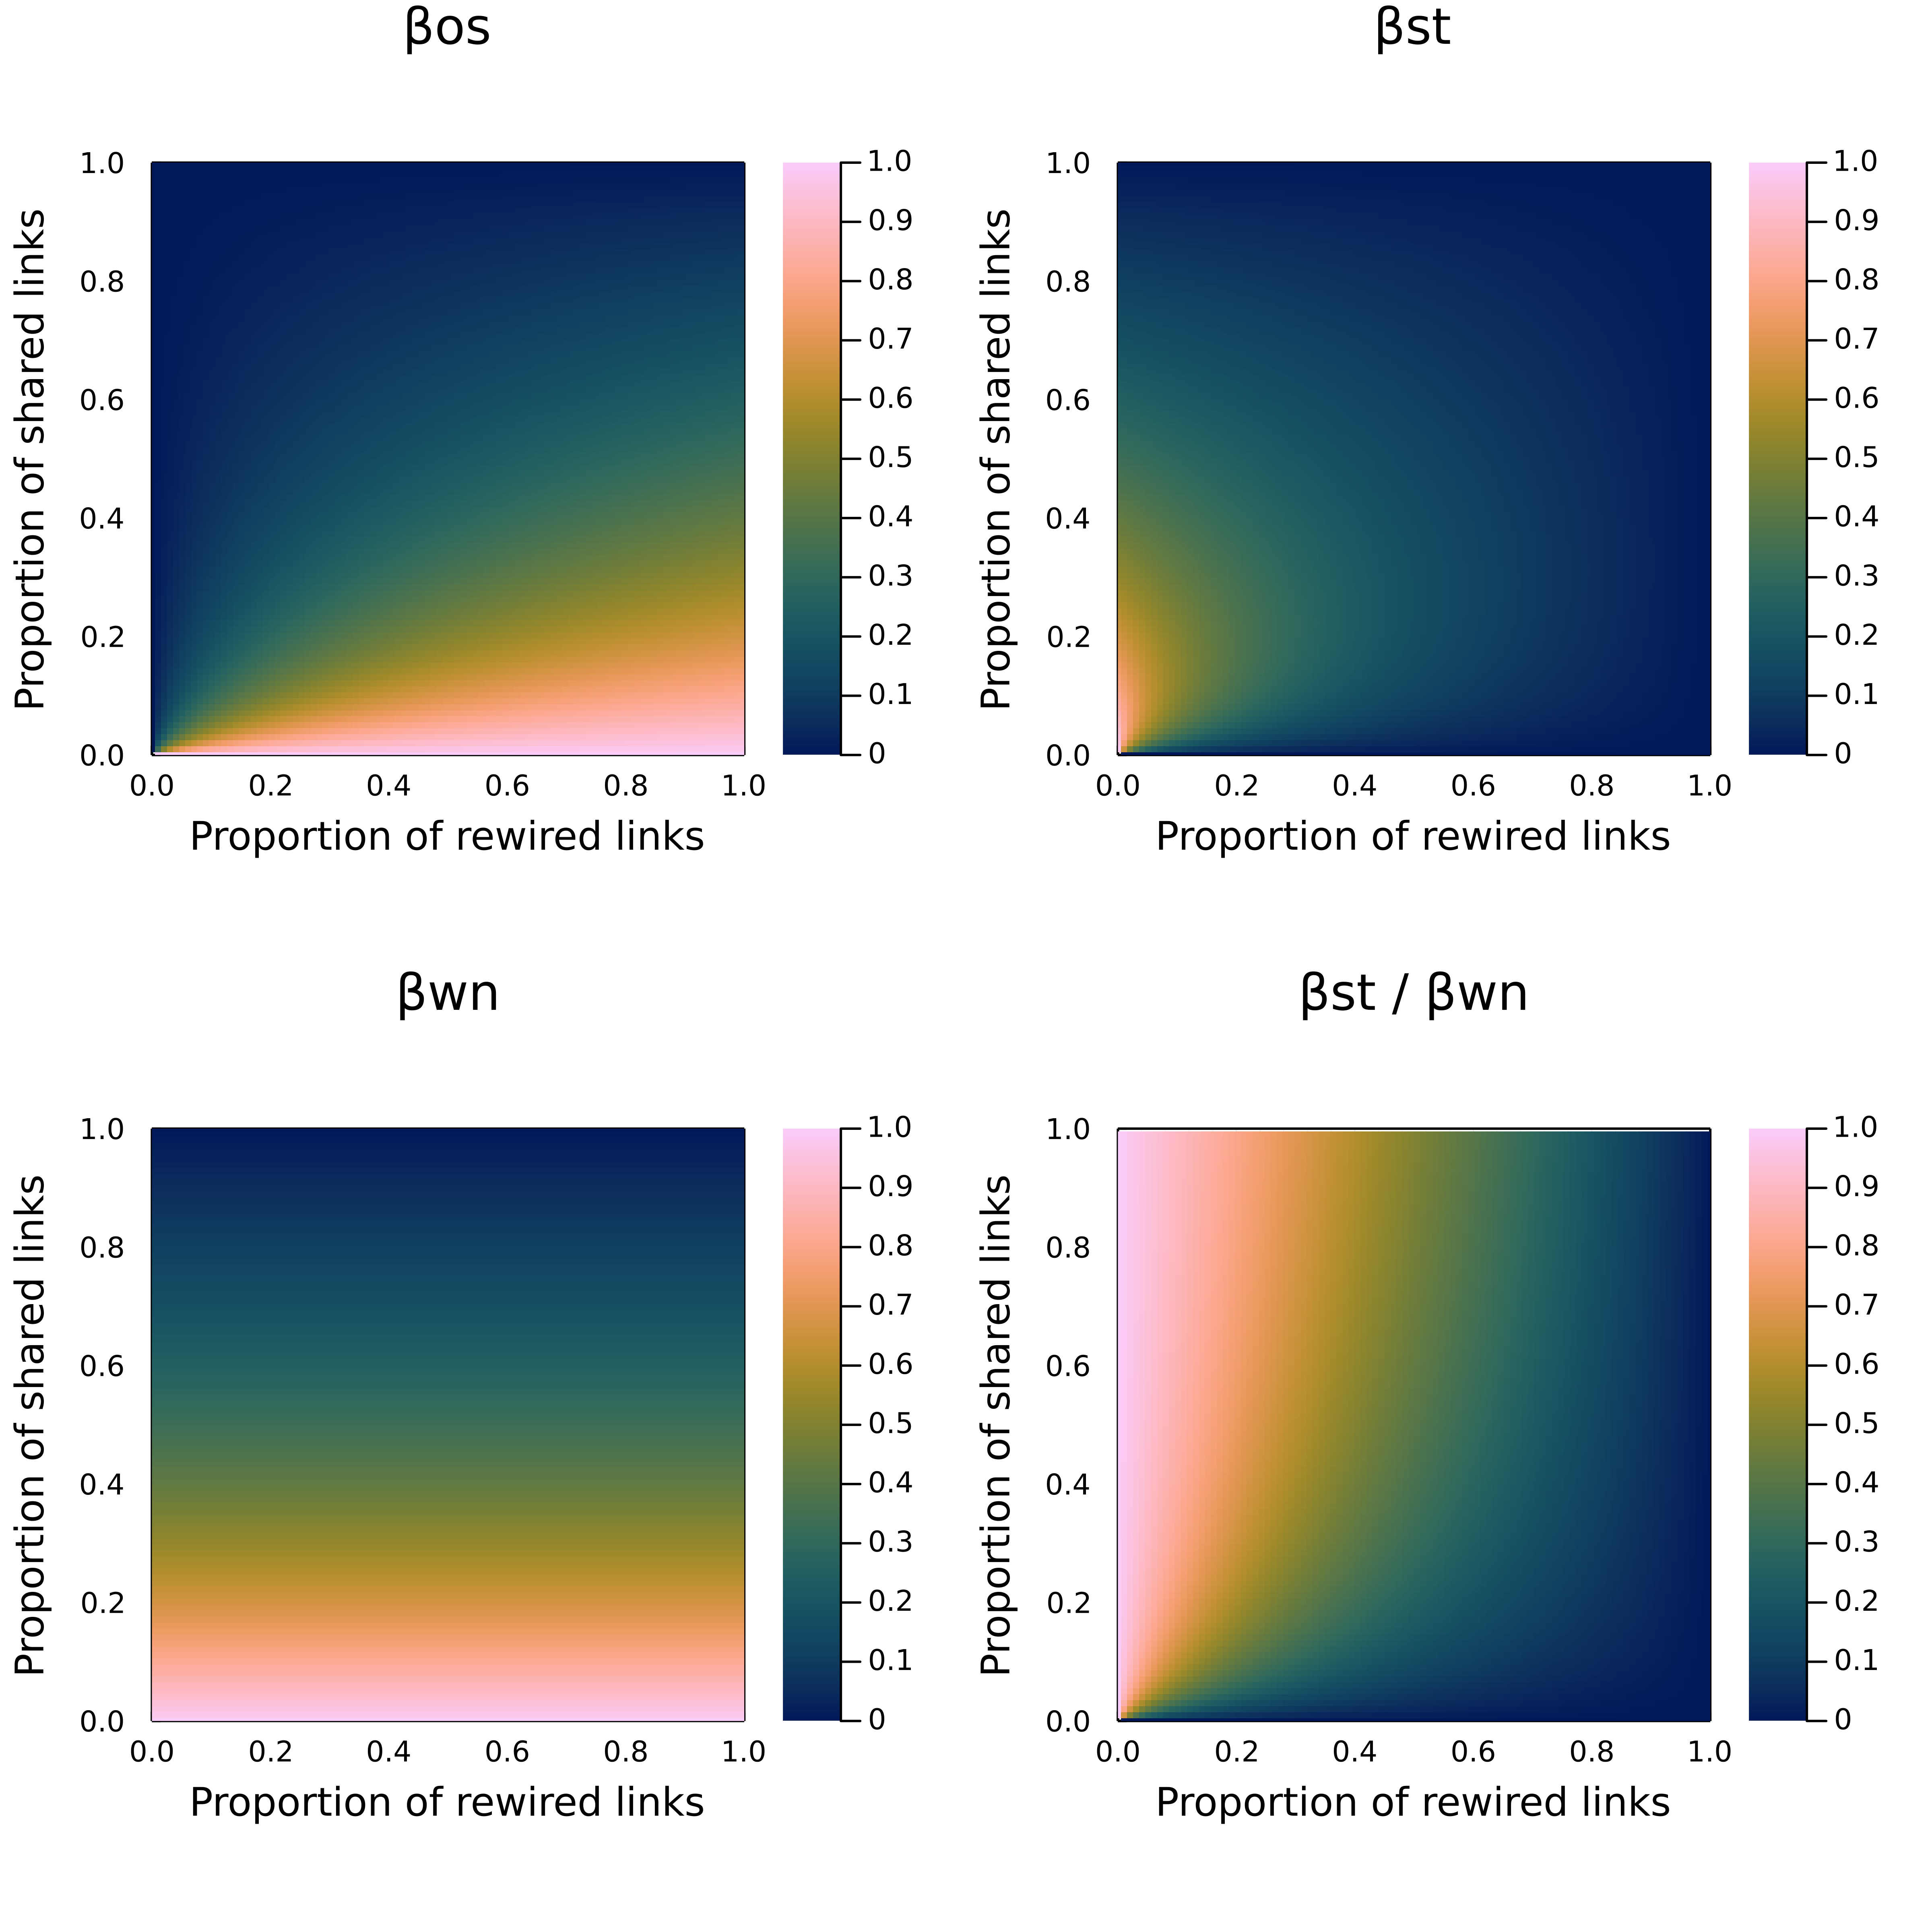
\includegraphics{figures/numexp1.png}
\caption{Values of \(\beta_{os}\), \(\beta_{wn}\), \(\beta_{st}\), and
\(\beta_{st}/\beta_{wn}\) as a function of the proportion of rewired
links and the proportion of shared links.}\label{fig:numexp1}
}
\end{figure}

The rewiring component \(\beta_{os}\) varies as a function of the
proportion of shared links that are rewired; by contrast, \(\beta_{wn}\)
varies \emph{only} as a function of the proportion of links that are
shared: that the unshared links are established between common or unique
species has no effect on overall network dissimilarity. The quadratic
nature of the denominator for \(\beta_{st}\) is clear here, with a
maximum reach when there is no re-wiring, and a small number of shared
links (\emph{i.e.} the networks are almost entirely dissimilar except
for the links between shared species). Althought the \emph{raw} values
of \(\beta_{st}\) may seem low, the normalization using
\(\beta_{st}/\beta_{wn}\) magnifies this effect: its values are indeed
maximized when the rewiring is lower, \emph{i.e.} all of the network
variation stems from turnover processes.

\hypertarget{is-this-decomposition-over-estimating-the-effect-of-rewiring}{%
\subsection{Is this decomposition over-estimating the effect of
``rewiring?''}\label{is-this-decomposition-over-estimating-the-effect-of-rewiring}}

One of the arguments put forth by Fründ (2021) is that the decomposition
outlined above will overestimate the effect of rewiring; I argue that
this is based on a misunderstanding of what \(\beta_{st}\) achieves. It
is paramount to clarify that \(\beta_{st}\) is not a direct measure of
the importance of turnover: it is a quantification of the relative
impact of rewiring to overall dissimilarity, which, all non-turnover
mechanisms being accounted for in the decomposition, can be explained by
turnover mechanisms. In this section, I present two numerical
experiments showing (i) that the \(\beta_{os}\) component is in fact an
accurate measure of rewiring, and (ii) that \(\beta_{st}\) captures the
consequences of species turnover, and of the interactions brought by
unique species.

\hypertarget{illustrations-on-arbitrarily-small-networks-are-biased}{%
\subsubsection{Illustrations on arbitrarily small networks are
biased}\label{illustrations-on-arbitrarily-small-networks-are-biased}}

We can re-calculate the illustration of Fründ (2021), wherein a pair of
networks with two shared interactions (\(A = 2\)) receive either an
interaction in \(S\), in \(U\), or in both:

\begin{longtable}[]{@{}lllllll@{}}
\toprule
\(A\) & \(S\) & \(U\) & \(\beta_{os}\) & \(\beta_{wn}\) & \(\beta_{st}\)
& \(\beta_{st}/\beta_{wn}\)\tabularnewline
\midrule
\endhead
2 & 0 & 0 & 0 & 0 & 0 &\tabularnewline
2 & 1 & 0 & \(1/5\) & \(1/5\) & 0 & 0\tabularnewline
2 & 0 & 1 & 0 & \(1/5\) & \(1/5\) & 0\tabularnewline
2 & 1 & 1 & \(1/5\) & \(1/3\) & \(2/15\) & \(2/5\)\tabularnewline
\bottomrule
\end{longtable}

The over-estimation argument hinges on the fact that
\(\beta_{st} < \beta_{os}\) in the last situation (one interaction as
rewiring, one as turnover). Reaching the conclusion of an overestimation
from this is based on a mis-interpretation of what \(\beta_{st}\) means.
The correct interpretation is that, out of the entire network
dissimilarity, only three-fifths are explained by re-wiring. The fact
that this fraction is not exactly one-half comes from the fact that the
Wilson \& Shmida (1984) measure counts shared interactions \emph{twice}
(\emph{i.e.} it has a \(2A\) term), which over-amplifies the effect of
shared interactions as the network is really small. Running the same
calculations with \(A = 10\) gives a relative importance of the turnover
processes of 47\%, and \(\beta_{st}\) goes to \(1/2\) as \(A/(S+U)\)
increases. As an additional caveat, the value of \(\beta_{st}\) will
depend on the measure of beta-diversity used. Measures that do not count
the shared interaction twice are not going to amplify the effect of
rewiring.

\hypertarget{numerical-experiment-the-decomposition-captures-the-roles-of-rewiring-and-turnover-accurately}{%
\subsubsection{Numerical experiment: the decomposition captures the
roles of rewiring and turnover
accurately}\label{numerical-experiment-the-decomposition-captures-the-roles-of-rewiring-and-turnover-accurately}}

Consider two bipartite networks, each with \(R\) species on either side,
and each with the same connectance \(\rho\). We will assume that these
networks \emph{share} a proportion \(p\) of their species from one side
(and share all species from the other), and that the interactions
between these species are undergo rewiring with at a rate \(q\). This is
sufficient information to calculate the values of \(A\), \(S\), and
\(U\) required to get the values of \(\beta_{os}\) and \(\beta_{wn}\).
Note that the simplification of assuming that only species from one side
can vary is merely for the sake of simplicity, but does not decrease the
generality of the argument.

Each network will have \(\rho(1-p)R^2\) interactions that are unique due
to species turnover, and so

\[U = 2\rho(1-p)R^2\,.\]

The part of both networks composed of overlapping species has
\(\rho pR^2\) interactions, of which \(\rho (1-q) p R^2\) are shared,
and \(\rho qp R^2\) underwent rewiring. This leads to

\[A = \rho (1-q) p R^2\,,\]

and

\[S = \rho pq R^2\,.\]

Note that we can drop the multiplicative constant \(R^2\), making the
result independent of the size of the network. Based on these
components, we can get the values of \(\beta_{os}\) and \(\beta_{wn}\),
as presented in fig.~\ref{fig:numexp2}.

\begin{figure}
\hypertarget{fig:numexp2}{%
\centering
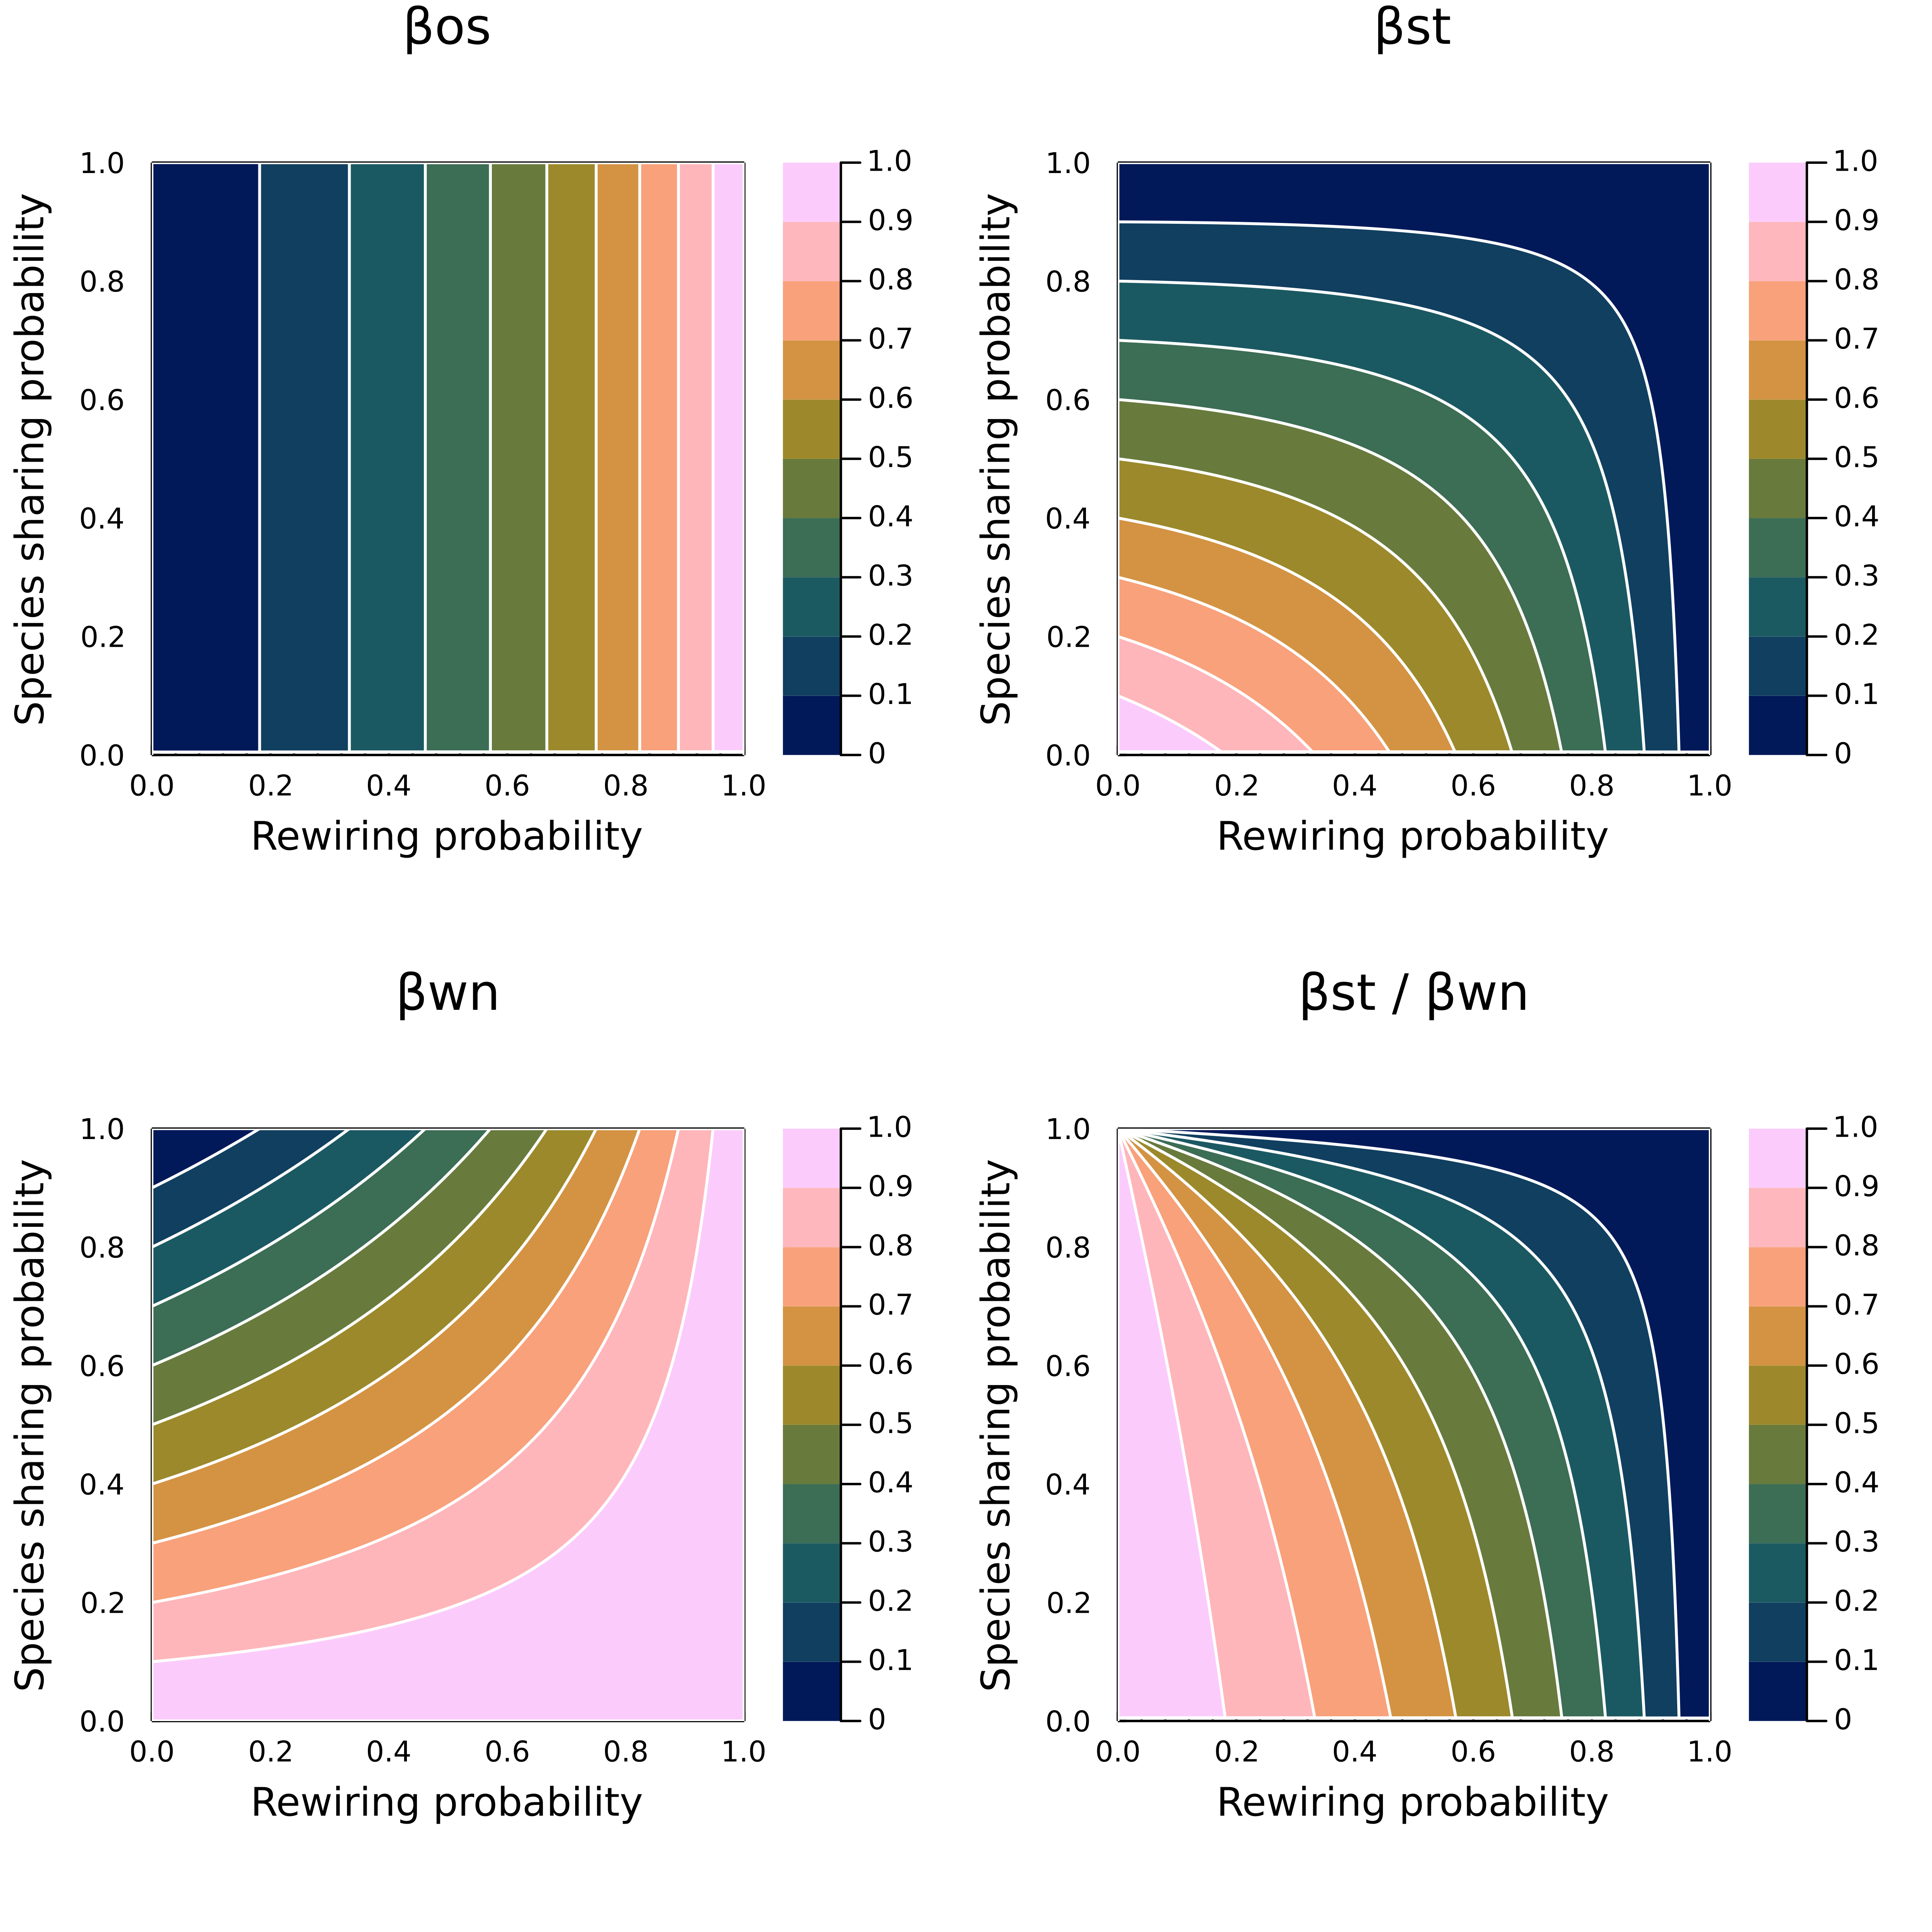
\includegraphics{figures/numexp2.png}
\caption{Response of \(\beta_{os}\) and \(\beta_{wn}\), and the
consequences on \(\beta_{st}\), to changes in rewiring probability
(\(q\)) and probability of species sharing (\(p\)). As expected,
\(\beta_{os}\) is not affected by species turnover, but increases with
the rewiring probability. By contrast, \(\beta_{wn}\) increases when the
rewiring probability is higher \emph{and} when fewer species are shared.
This has important consequences for \(\beta_{st}\): its value is
maximized for low species sharing, and decreases for high rewiring
probability.}\label{fig:numexp2}
}
\end{figure}

The value of \(\beta_{os}\) is entirely unchanged by variations in \(p\)
(species sharing), and responds \emph{only} to changes in \(q\) (the
probability of rewiring), whereas as expected, \(\beta_{wn}\) responded
to changes in both of these parameters: the most dissimilar networks
have low species sharing (interactions are dissimilar because brought by
unique species), and high rewiring (shared species do not share
interactions). The relative changes in \(\beta_{os}\) and \(\beta_{wn}\)
lead to predictable changes in \(\beta_{st}\): its value is maximized
when both rewiring \emph{and} species sharing are low. Increasing
rewiring decreases the impact of species turnover (because, for an equal
number of interactions, the dissimilarity of interactins in shared
species contributes more to \(\beta_{wn}\)); increasing the chance of
sharing species also does decrease \(\beta_{st}\), trivially because
there is no species turnover anymore. Note that when using the
correction of \(\beta_{st}/\beta_{wn}\), the effect of species turnover
is magnified for low probabilities of re-wiring.

In conclusion, this numerical experiment shows that the decomposition as
initially presented by Poisot \emph{et al.} (2012), \emph{i.e.} using
denominators that make sense from a network composition point of view,
succeeds at capturing the relative effect of turnover and rewiring.

\hypertarget{numerical-experiment-the-decomposition-captures-the-roles-of-species-turnover-and-connectance-accurately}{%
\subsubsection{Numerical experiment: the decomposition captures the
roles of species turnover and connectance
accurately}\label{numerical-experiment-the-decomposition-captures-the-roles-of-species-turnover-and-connectance-accurately}}

Consider now two bipartite networks, which still have \(R\) species on
either side, but differ in their connectance (\(\rho_1\) and \(\rho_2\))
-- by maintaining the assumption that species on one side are shared
with probability \(p\), and that interactions between shared species are
rewired at probability \(q\), we can examine the effect of varying both
connectance and turnover on the value of the \(\beta\)-diversity
components. Note that, although not presented, we will drop the
multiplicative constant \(R^2\) from all calculations, as it is a common
factor for all values; again, this implies that the results presented
here are independant of network richness.

The number of unique links due to species turnover is

\[U = (1-p)(\rho_1 + \rho_2)\,,\]

which decreases with the proportion of shared species, but increases
with connectance. The number of links between shared species takes a
little more steps to calculate. First, amongst the \(pR^2\) species in
both sub-graphs, network 1 will have \(\rho_1 pR^2\), and network 2 will
have \(\rho_2 pR^2\). Because \(\rho_1 \neq \rho_2\), there are only
\(\text{min}(\rho_1, \rho_2)pR^2\) links that can be shared, a
proportion \(q\) of which will undergo re-wiring, and a proportion
\((1-q)\) of which will be shared. This leads to the expression (after
dropping \(R^2\)) for the number of shared links:

\[A = p (1-q) \text{min}(\rho_1, \rho_2)\,.\]

The number of unique links due to shared species is the sum of all links
in network 1 (\(\rho_1 R^2\)), minus the sum of the shared links
(\(AR^2\)) and the unique links due to species turnover
(\((1-p)\rho_1R^2\)); this same quantity is calculated in the same way
for the second networks, leading to (after dropping the multiplicative
constant \(R^2\) and some simplifications)

\[S = p (\rho_1 + \rho_2) - 2A\,.\]

Note that as expected, this last quantity scales with the proportion of
shared species (\(p\)) \emph{and} with connectance (as shared species
bring more of their interactions), but decreases with the size of the
shared links components. The consequences of varying \(\rho_2\) and
\(p\) are presented in fig.~\ref{fig:numexp3}.

\begin{figure}
\hypertarget{fig:numexp3}{%
\centering
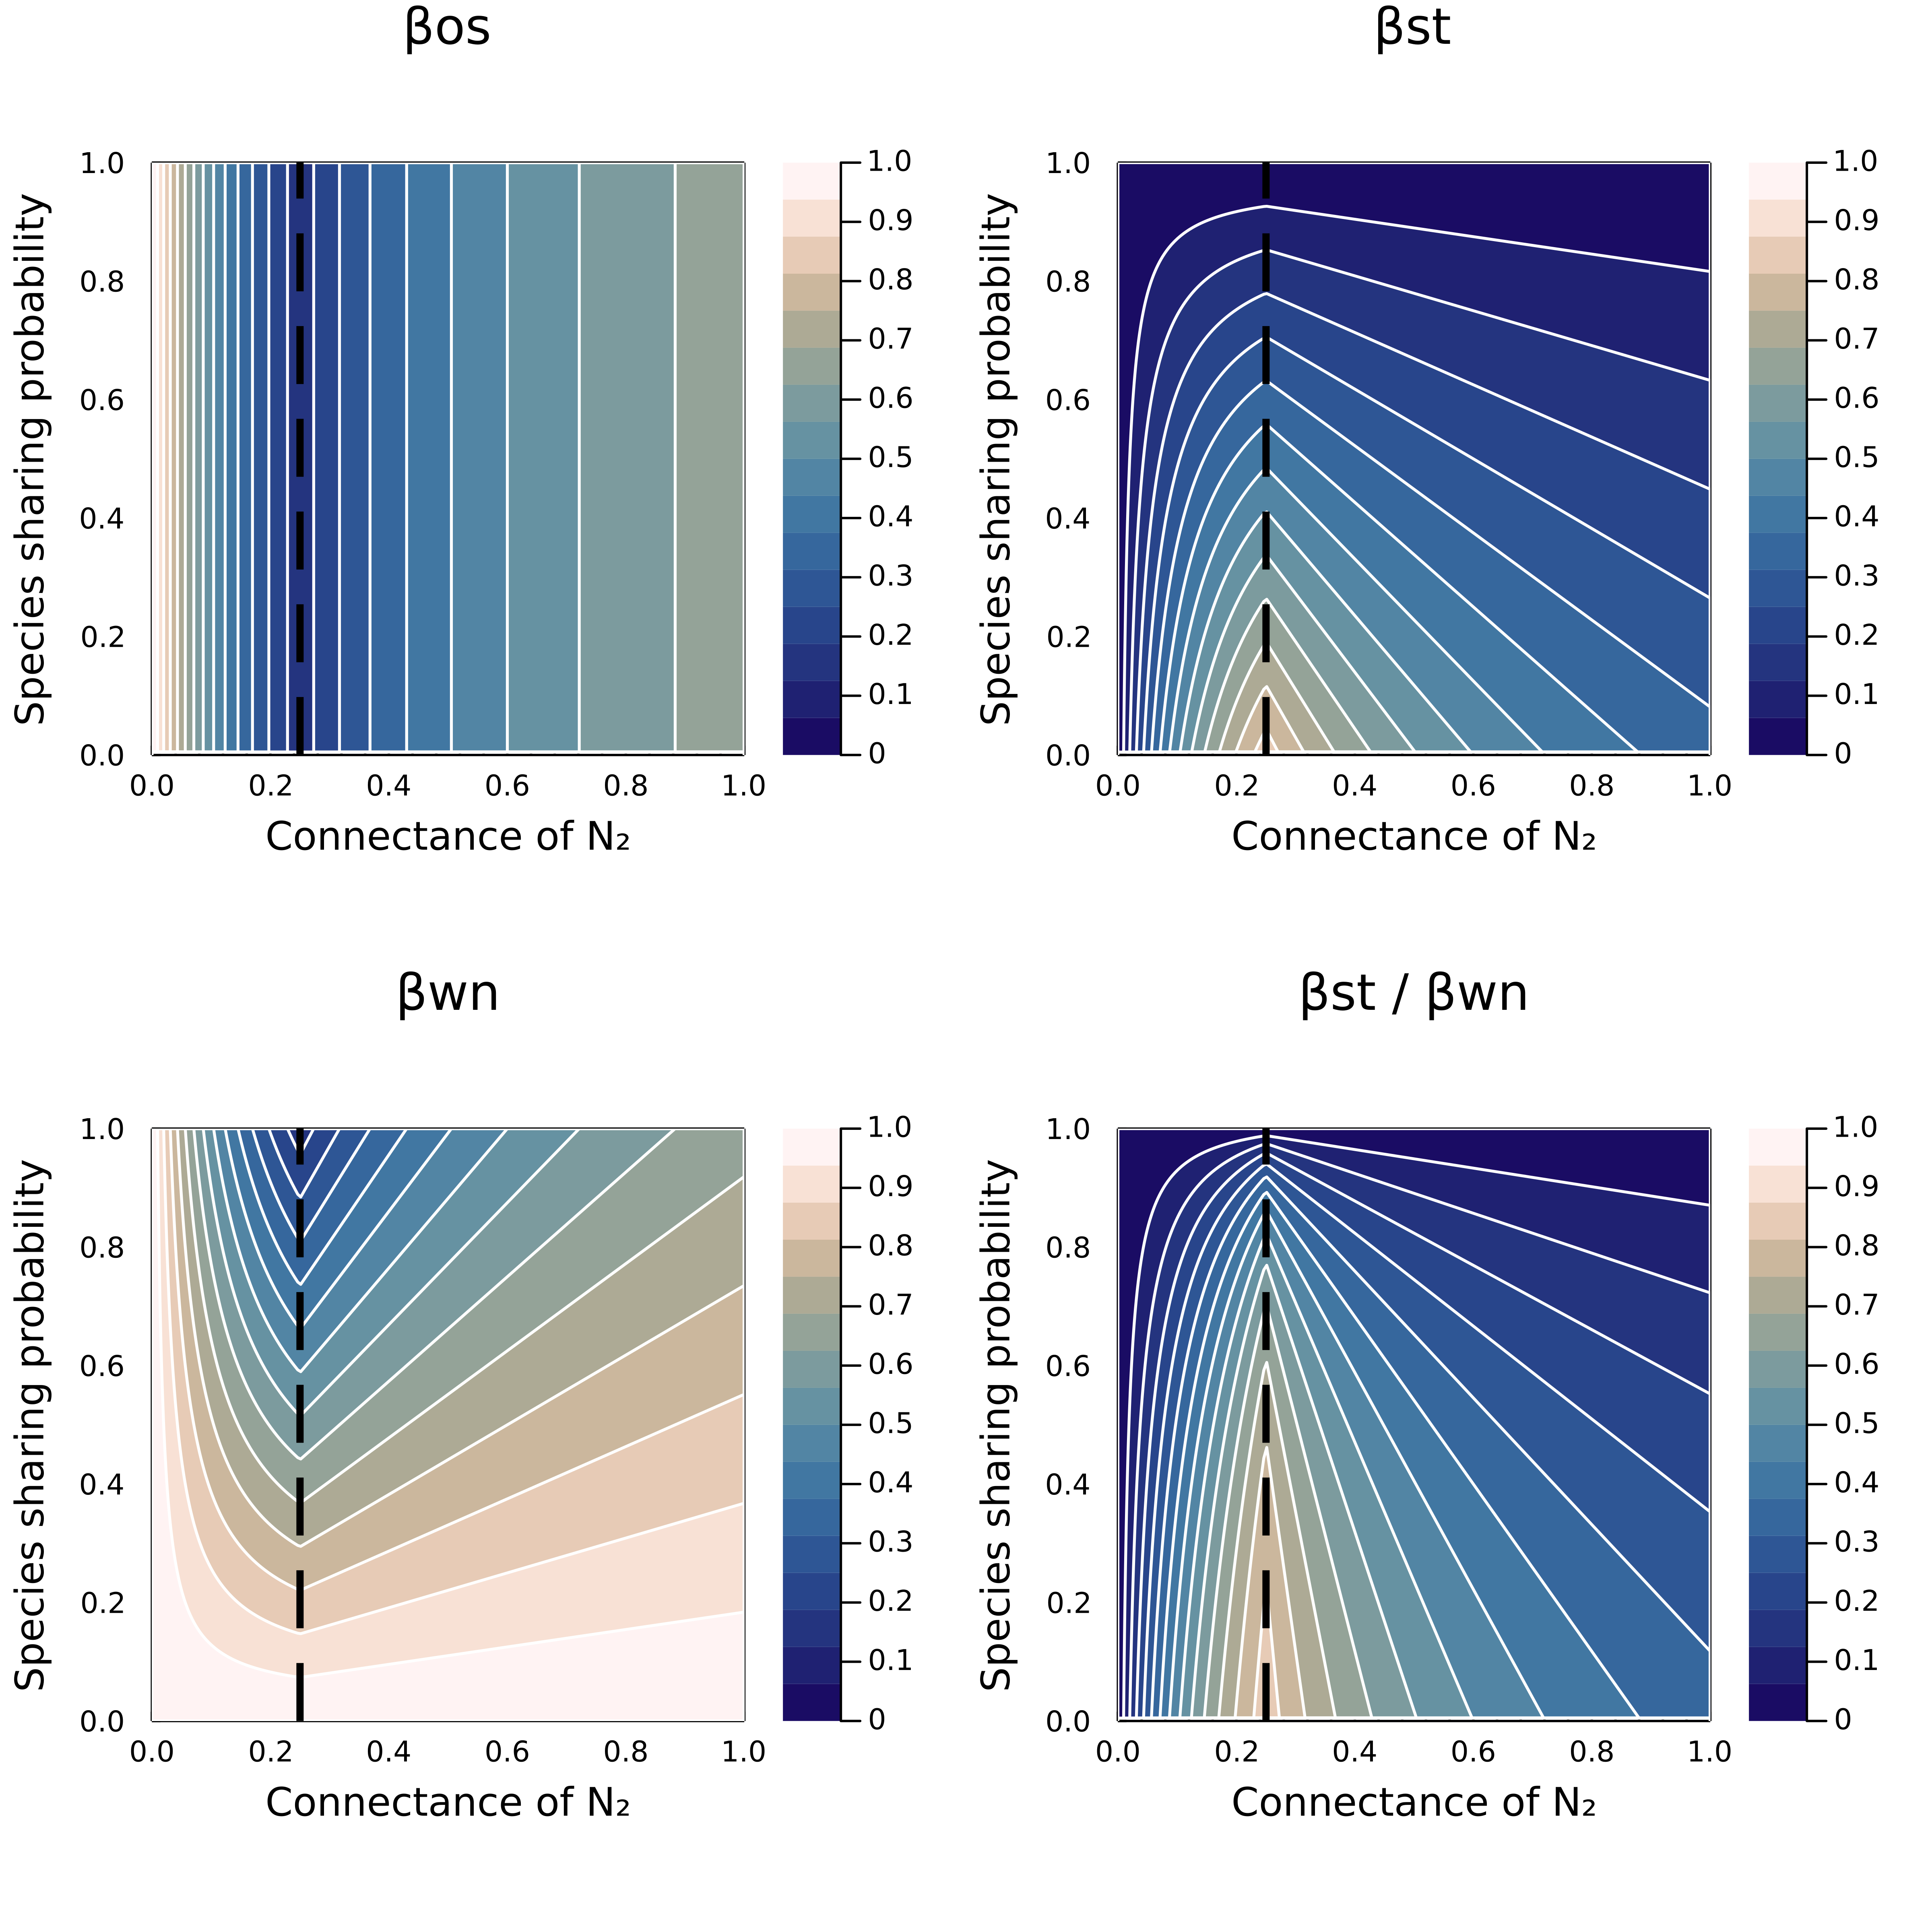
\includegraphics{figures/numexp3.png}
\caption{Effects of varying the connectance of the second network
(\(\rho_2\)) and the proportion of shared species (\(p\)) on the values
of the \(\beta\)-diversity components. As expected, \(\beta_{os}\) is
still independent of species turnover, and \(\beta_{wn}\) increases when
species turnover increases, or when the connectances become more
dissimilar. These figures have been generated with \(\rho_1 = 0.25\) and
\(q = 0.15\), and the results are qualitatively robust to changes in
these parameters.}\label{fig:numexp3}
}
\end{figure}

Although \(\beta_{os}\) is only responding to changes in connectance (as
is expected, seeing that the relative connectances of both networks
appear in the expression for \(S\) and \(A\)), \(\beta_{wn}\) changes in
response to both parameters. Specifically, increasing the difference in
connectance between the two networks, especially when also increasing
the species dissimilarity, results in more dissimilar networks -- this
is because unique species from both networks bring their own
interactions (at rate \(\rho_1\) and \(\rho_2\)), and therefore
contribute to dissimilarity. It is particularly noteworthy that
\(\beta_{st}\), regardless of the differences in connectance, increases
with the proportion of unique species. At an equal proportion of shared
species, \(\beta_{st}\) \emph{decreases} with differences in
connectance: this is an equally expected result, which indicates that
the difference between \(\beta_{os}\) and \(\beta_{wn}\) is in part
explained by non-turnover mechanisms (here, changes in connectance).
Relying on the \(\beta_{st}/\beta_{wn}\) correction again magnifies this
effect, without changing their interpretation.

\hypertarget{does-the-partition-of-network-dissimilarity-needs-a-new-normalization}{%
\subsection{Does the partition of network dissimilarity needs a new
normalization?}\label{does-the-partition-of-network-dissimilarity-needs-a-new-normalization}}

Based on the arguments presented above, I do not think the suggestion of
Fründ (2021) to change the denominator of \(\beta_{os}\) makes sense as
a default; the strength of the original approach by Poisot \emph{et al.}
(2012) is indeed that the effect of turnover is based on a rigorous
definition of networks as graphs (as opposed to networks as matrices),
in which the induction of vertices from the edgelist being compared
gives rise to biologically meaningful denominators. The advantage of
this approach is that at no time does the turnover of species itself (or
indeed, as shown in many places in this manuscript, the network
richness), or the connectance of the network, enter into the
calculation. As such, it is possible to use \(\beta_{os}\) and
\(\beta_{wn}\) in relationship to these terms, calculated externally (as
was recently done by \emph{e.g.} Higino \& Poisot 2021), without
creating circularities.

The choice of changing the denominator hinges on what one admits as a
definition for \(\beta_{st}\). If the point of \(\beta_{st}\) is to be a
component of overall \(\beta\)-diversity as advocated by Fründ (2021)
and Novotny (2009), a change of numerator \emph{might} be acceptable.
Nevertheless, this change of numerator contributes to blurring the
frontier between a measure of interaction dissimilarity and a measure of
community dissimilarity which starts to add the effect of relative
richness; this later case warrants a thorough methodological assessment.
Conversely, if as we argue in Poisot \emph{et al.} (2012),
\(\beta_{st}\) is to be meant as a \emph{guide} to the interpretation of
\(\beta_{wn}\) and \(\beta_{os}\), and related to actual measures of
species turnover and network connectance, one must not change the
denominator.

It is essential to recognize that there are multiple reasons to
calculate network dissimilarity, and it is our opinion that the
arguments levied by Fründ (2021) against the original partition stem
from a misunderstanding of what it intends to do (and does, indeed, do
well), not from intrinsic methodological issues in the partition itself.
Based on the results presented in this contribution, I argue that the
original partition of network \(\beta\)-diversity from Poisot \emph{et
al.} (2012) should remain the default.

\hypertarget{references}{%
\subsection*{References}\label{references}}
\addcontentsline{toc}{subsection}{References}

\hypertarget{refs}{}
\begin{CSLReferences}{1}{0}
\leavevmode\hypertarget{ref-Banville2021ManJl}{}%
Banville, F., Vissault, S. \& Poisot, T. (2021). Mangal.jl and
EcologicalNetworks.jl: Two complementary packages for analyzing
ecological networks in Julia. \emph{Journal of Open Source Software}, 6,
2721.

\leavevmode\hypertarget{ref-Baronio2021NatFir}{}%
Baronio, G.J., Souza, C.S., Maruyama, P.K., Raizer, J., Sigrist, M.R. \&
Aoki, C. (2021). Natural fire does not affect the structure and beta
diversity of plant-pollinator networks, but diminishes floral-visitor
specialization in Cerrado. \emph{Flora}, 281, 151869.

\leavevmode\hypertarget{ref-Campos-Moreno2021ImpInt}{}%
Campos-Moreno, D.F., Dyer, L.A., Salcido, D., Massad, T.J.,
Pérez-Lachaud, G., Tepe, E.J., \emph{et al.} (2021). Importance of
interaction rewiring in determining spatial and temporal turnover of
tritrophic (Piper-caterpillar-parasitoid) metanetworks in the Yucatán
Península, México. \emph{Biotropica}, 53, 1071--1081.

\leavevmode\hypertarget{ref-Canard2014EmpEva}{}%
Canard, E.F., Mouquet, N., Mouillot, D., Stanko, M., Miklisova, D. \&
Gravel, D. (2014). Empirical evaluation of neutral interactions in
host-parasite networks. \emph{The American Naturalist}, 183, 468--479.

\leavevmode\hypertarget{ref-Dunne2006NetStr}{}%
Dunne, J.A. (2006). The Network Structure of Food Webs. In:
\emph{Ecological networks: Linking structure and dynamics} (eds. Dunne,
J.A. \& Pascual, M.). Oxford University Press, pp. 27--86.

\leavevmode\hypertarget{ref-Frund2021DisSpe}{}%
Fründ, J. (2021). Dissimilarity of species interaction networks: How to
partition rewiring and species turnover components. \emph{Ecosphere},
12, e03653.

\leavevmode\hypertarget{ref-Higino2021BetPhy}{}%
Higino, G.T. \& Poisot, T. (2021). Beta and phylogenetic diversities
tell complementary stories about ecological networks biogeography.
\emph{Parasitology}, 1--23.

\leavevmode\hypertarget{ref-Koleff2003MeaBet}{}%
Koleff, P., Gaston, K.J. \& Lennon, J.J. (2003). Measuring beta
diversity for presence--absence data. \emph{Journal of Animal Ecology},
72, 367--382.

\leavevmode\hypertarget{ref-Legendre2013BetDiv}{}%
Legendre, P. \& De Cáceres, M. (2013). Beta diversity as the variance of
community data: Dissimilarity coefficients and partitioning.
\emph{Ecology Letters}, 16, 951--963.

\leavevmode\hypertarget{ref-Magrach2017PlaNet}{}%
Magrach, A., Holzschuh, A., Bartomeus, I., Riedinger, V., Roberts,
S.P.M., Rundlöf, M., \emph{et al.} (2017). Plant-pollinator networks in
semi-natural grasslands are resistant to the loss of pollinators during
blooming of mass-flowering crops. \emph{Ecography}, n/a--n/a.

\leavevmode\hypertarget{ref-Novotny2009BetDiv}{}%
Novotny, V. (2009). Beta diversity of plant--insect food webs in
tropical forests: A conceptual framework. \emph{Insect Conservation and
Diversity}, 2, 5--9.

\leavevmode\hypertarget{ref-Olsson2021IntPla}{}%
Olsson, R.L., Brousil, M.R., Clark, R.E., Baine, Q. \& Crowder, D.W.
(2021). Interactions between plants and pollinators across urban and
rural farming landscapes. \emph{Food Webs}, 27, e00194.

\leavevmode\hypertarget{ref-Poisot2012DisSpe}{}%
Poisot, T., Canard, E., Mouillot, D., Mouquet, N. \& Gravel, D. (2012).
The dissimilarity of species interaction networks. \emph{Ecology
Letters}, 15, 1353--1361.

\leavevmode\hypertarget{ref-Poisot2016StrPro}{}%
Poisot, T., Cirtwill, A.R., Cazelles, K., Gravel, D., Fortin, M.-J. \&
Stouffer, D.B. (2016). The structure of probabilistic networks.
\emph{Methods in Ecology and Evolution}, 7, 303--312.

\leavevmode\hypertarget{ref-Poisot2017HosPar}{}%
Poisot, T., Gueveneux-Julien, C., Fortin, M.-J., Gravel, D. \& Legendre,
P. (2017). Hosts, parasites and their interactions respond to different
climatic variables. \emph{Global Ecology and Biogeography}, n/a--n/a.

\leavevmode\hypertarget{ref-Poisot2015SpeWhy}{}%
Poisot, T., Stouffer, D.B. \& Gravel, D. (2015). Beyond species: Why
ecological interaction networks vary through space and time.
\emph{Oikos}, 124, 243--251.

\leavevmode\hypertarget{ref-Souza2021PlaSam}{}%
Souza, C.S., Maruyama, P.K., Santos, K.C.B.S., Varassin, I.G., Gross,
C.L. \& Araujo, A.C. (2021). Plant-centred sampling estimates higher
beta diversity of interactions than pollinator-based sampling across
habitats. \emph{New Phytologist}, 230, 2501--2512.

\leavevmode\hypertarget{ref-Trojelsgaard2016EcoNet}{}%
Trøjelsgaard, K. \& Olesen, J.M. (2016). Ecological networks in motion:
Micro- and macroscopic variability across scales. \emph{Functional
Ecology}, 30, 1926--1935.

\leavevmode\hypertarget{ref-Tuomisto2010DivBet}{}%
Tuomisto, H. (2010). A diversity of beta diversities: Straightening up a
concept gone awry. Part 1. Defining beta diversity as a function of
alpha and gamma diversity. \emph{Ecography}, 33, 2--22.

\leavevmode\hypertarget{ref-Wilson1984MeaBet}{}%
Wilson, M.V. \& Shmida, A. (1984). Measuring Beta Diversity with
Presence-Absence Data. \emph{Journal of Ecology}, 72, 1055--1064.

\end{CSLReferences}

\end{document}
